\documentclass{tktltiki}
\usepackage{url}
\usepackage{graphicx}
\begin{document}
\title{Keskitetty tunnistautuminen web-sovelluksissa}
\author{Olli Jokinen}
\date{\today}
\level{Pro gradu -tutkielma}
\maketitle
\doublespacing
\faculty{Matemaattis-luonnontieteellinen}
\department{Tietojenkäsittelytieteen laitos}
\subject{Tietojenkäsittelytiede}
\depositeplace{Tietojenkäsittelytieteen laitoksen kirjasto}
\additionalinformation{}
\numberofpagesinformation{\numberofpages\ sivua +
\numberofappendixpages[100] liitesivua}
\classification{A.1 [Introductory and Survey] \\
I.7.m [Document and Text Processing]: Miscellaneous}
\keywords{avainsana}
\begin{abstract}
Tutkielmassa selvitetään keskitetyn tunnistautumispalvelun toteuttamista palveluperustaisten arkkitehtuurien mukaisissa web-sovellusympäristöissä. Painopisteenä ovat sovellusympäristöt, joissa ollaan siirtymässä palveluperustaisiin arkkitehtuureihin. Tutkielmassa käytetään esimerkkinä tällaisesta ympäristöstä Kapsi Internet-käyttäjät ry:n jäsenhallintatyökaluja, joiden tunnistautuminen muutetaan keskitetyn tunnistautumispalvelun tehtäväksi.

Ensimmäiseksi tutkielmassa esitellään web-sovellusten kehitys varhaisista CGI-ohjelmista kohti palveluperustaisten arkkitehtuurien mukaisia web-sovelluksia ja esitellään tunnistautumisen tarpeet tällaisissa arkkitehtuureissa sekä käydään läpi turvallisuuden osatekijöitä ja tavallisia tunnistautumiseen liittyviä ongelmia web-sovelluksissa. Seuraavaksi hahmotellaan tunnistautumisongelman ratkaisuun tarkoitettu keskitetty tunnistautumispalvelu sekä pohditaan sen etuja ja haittoja verrattuna nykyisin yleisesti käytettyihin tunnistautumismekanismeihin.

Sitten tutkitaan tunnistautumispalvelun ja web-sovelluksen väliseen rajapintaan käytettäviä protokollia (SAML, OpenID ja OAuth) ja esitellään OAuth-protokollaa käyttävä Kapsin web-sovellusarkkitehtuuri. Esitetyn arkkitehtuurin etuja ja haittoja sekä sen soveltamista muihin vastaaviin ympäristöihin tutkitaan myös. Arkkitehtuurin laajentamista keskitettyyn pääsynvalvontaan ja kertakirjautumiseen pohditaan tutkielman loppupuolella. Lopuksi pohditaan ulkoisen tunnistautumispalvelun käyttöä, esimerkkinä käytetään Facebookin tarjoamaa tunnistautumisrajapintaa.
\end{abstract}
\mytableofcontents
\section{Johdanto}
Tunnistautumiseen liittyvien käsitteiden läpikäynti ennen protokollien yksityiskohtaista esittelyä auttaa tunnistautumiseen liittyvien periaatteiden hahmottamista. Käsitteet ovat yleisluontoisia ja eivätkä kosketa vain tiettyjä protokollaa. Protokollien yhteydessä käytetään käsitteitä asiakasohjelma, tunnistautumispalvelu, suojattu resurssi, valtuutustieto (credentials), valtuutusavain (authorization code) ja pääsyvaltuutus (access token) \cite{nisti}.

Asiakasohjelmalla tarkoitetaan web-palvelun käyttäjän pääteohjelmaa, jolla hän kirjautuu web-palveluun käyttäen keskitettyä tunnistautumispalvelua. Käytännössä asiakasohjelma on web-palvelun tapauksessa käyttäjän WWW-selain, joka pystyy tekemään uudelleenohjauksia sivustolta toiselle. Uudelleenohjaus on HTTP-protokollan perustoiminnallisuutta, joten mikä tahansa HTTP/1.1-standardin WWW-selain käy asiakasohjelmaksi \cite{rfc2616}.

Tunnistautumispalvelu on web-palvelu, johon käyttäjä ohjataan tekemään tunnistautuminen. Onnistuneen tunnistautumisen jälkeen tunnistautumispalvelu ohjaa asi\-a\-kas\-oh\-jel\-man takaisin tunnistautumista pyytäneen palvelun määrittelemään osoitteeseen \cite{nisti}. Avoimen Internetin puolella tunnistautumispalvelu voi olla esimerkiksi Facebook tai LinkedIn.

Tunnistautumisprotokollien yhteydessä suojatulla resurssilla tarkoitetaan resurssia, jonka käyttö vaatii tunnistautumisen ja käyttöoikeuden. Yleisessä tapauksessa suojatulla resurssilla tarkoitetaan yksittäistä resurssia (käyttäjän valokuvaa), johon halutaan asettaa pääsyrajoituksia \cite{nisti}. Tämän tutkielman puitteissa suojatulla resurssilla tarkoitetaan tunnistautumista vaativaa web-palvelua.

Valtuutustieto koostuu yksilöivästä tunnisteesta ja siihen liittyvästä salaisesta avaimesta. Tämän tutkielman puitteissa valtuutustiedolla tarkoitetaan käyttäjän tunnusta ja salasanaa.

Kirjauduttuaan sisään tunnistautumispalvelimelle, käyttäjä saa valtuutusavaimen, jonka hän lähettää eteenpäin suojatun resurssin omistajalle. Valtuutusavain ei pidä sisällään käyttäjän valtuutustietoja, vaan ainoastaan tunnistautumispalvelin osaa lukea sen \cite{nisti}. Saatuaan valtuutusavaimen käyttäjältä voi suojatun resurssin omistaja hakea pääsyvaltuuden käyttäjän tietoihin tunnistautumispalvelusta.

Pääsyvaltuutus on tunnistautumispalvelimelta saatava yksilöivä tunniste, jonka avulla suojatun resurssin omistaja voi pyytää käyttäjän tiedot tunnistautumispalvelulta. Pääsyvaltuutus on voimassa tietyn ajan, jonka jälkeen se täytyy uusia tunnistautumispalvelimella \cite{nisti}. Pääsyvaltuutusta voidaan käyttää myös tunnistautumispalvelusta erillään olevien resurssien valtuuttamiseen. Esimerkiksi web-sovellus voi hakea tunnistautumispalvelulta pääsyvaltuuden, jolla hän hakee valokuvia valokuvien jakopalvelusta \cite{facebook}.
\section{Web-sovellukset}
Tunnistautumiseen liittyvien käsitteiden läpikäynti ennen protokollien yksityiskohtaista esittelyä auttaa tunnistautumiseen liittyvien periaatteiden hahmottamista. Käsitteet ovat yleisluontoisia ja eivätkä kosketa vain tiettyjä protokollaa. Protokollien yhteydessä käytetään käsitteitä asiakasohjelma, tunnistautumispalvelu, suojattu resurssi, valtuutustieto (credentials), valtuutusavain (authorization code) ja pääsyvaltuutus (access token) \cite{nisti}.

Asiakasohjelmalla tarkoitetaan web-palvelun käyttäjän pääteohjelmaa, jolla hän kirjautuu web-palveluun käyttäen keskitettyä tunnistautumispalvelua. Käytännössä asiakasohjelma on web-palvelun tapauksessa käyttäjän WWW-selain, joka pystyy tekemään uudelleenohjauksia sivustolta toiselle. Uudelleenohjaus on HTTP-protokollan perustoiminnallisuutta, joten mikä tahansa HTTP/1.1-standardin WWW-selain käy asiakasohjelmaksi \cite{rfc2616}.

Tunnistautumispalvelu on web-palvelu, johon käyttäjä ohjataan tekemään tunnistautuminen. Onnistuneen tunnistautumisen jälkeen tunnistautumispalvelu ohjaa asi\-a\-kas\-oh\-jel\-man takaisin tunnistautumista pyytäneen palvelun määrittelemään osoitteeseen \cite{nisti}. Avoimen Internetin puolella tunnistautumispalvelu voi olla esimerkiksi Facebook tai LinkedIn.

Tunnistautumisprotokollien yhteydessä suojatulla resurssilla tarkoitetaan resurssia, jonka käyttö vaatii tunnistautumisen ja käyttöoikeuden. Yleisessä tapauksessa suojatulla resurssilla tarkoitetaan yksittäistä resurssia (käyttäjän valokuvaa), johon halutaan asettaa pääsyrajoituksia \cite{nisti}. Tämän tutkielman puitteissa suojatulla resurssilla tarkoitetaan tunnistautumista vaativaa web-palvelua.

Valtuutustieto koostuu yksilöivästä tunnisteesta ja siihen liittyvästä salaisesta avaimesta. Tämän tutkielman puitteissa valtuutustiedolla tarkoitetaan käyttäjän tunnusta ja salasanaa.

Kirjauduttuaan sisään tunnistautumispalvelimelle, käyttäjä saa valtuutusavaimen, jonka hän lähettää eteenpäin suojatun resurssin omistajalle. Valtuutusavain ei pidä sisällään käyttäjän valtuutustietoja, vaan ainoastaan tunnistautumispalvelin osaa lukea sen \cite{nisti}. Saatuaan valtuutusavaimen käyttäjältä voi suojatun resurssin omistaja hakea pääsyvaltuuden käyttäjän tietoihin tunnistautumispalvelusta.

Pääsyvaltuutus on tunnistautumispalvelimelta saatava yksilöivä tunniste, jonka avulla suojatun resurssin omistaja voi pyytää käyttäjän tiedot tunnistautumispalvelulta. Pääsyvaltuutus on voimassa tietyn ajan, jonka jälkeen se täytyy uusia tunnistautumispalvelimella \cite{nisti}. Pääsyvaltuutusta voidaan käyttää myös tunnistautumispalvelusta erillään olevien resurssien valtuuttamiseen. Esimerkiksi web-sovellus voi hakea tunnistautumispalvelulta pääsyvaltuuden, jolla hän hakee valokuvia valokuvien jakopalvelusta \cite{facebook}.
\subsection{Tunnistautumisen historia}
WWW:n, ja erityisesti sen edeltäjän Gopherin, sivustot olivat alkujaan lähinnä staattisia dokumentteja, jotka oli linkitetty toisiinsa. Dokumentit muodostivat erillisia arkistoja esimerkiksi tutkijoiden käyttöön. Ajan kuluessa tuli tarpeelliseksi tehdä sivustoja, jotka reagoivat käyttäjän syötteeseen ja toimivat dynaamisesti syötteen mukaan \cite{dynamic}.

Vuonna 1993 esitelty Common Gateway Interface (CGI) on standardi, jolla voidaan suorittaa ohjelmia web-sivujen kautta UNIX-ympäristössä \cite{rfc3875}. Tyypillisesti CGI:llä suoritettavat ohjelmat ovat itsenäisiä ja kirjoitettu jollain skriptikielellä, esimerkiksi Perlillä tai PHP:lla. Skripti saa parametrina käyttäjän lähettämät syötteet ja muodostaa sen perusteella käyttäjälle näkyvän HTML-sivun. Ajan kuluessa CGI-ohjelmat alkoivat kasvaa ja niiden arkkitehtuuri monimutkaistua, kun sovelluksissa käsiteltävät tietomäärät alkoivat vaatia tietokantoja.

CGI-ohjelmien kasvun lisäksi myös niiden suoritukseen vaadittava ajoympäristö alkoi kasvaa, mikä muodostaa ongelmia CGI:n käytölle. CGI käynnistää suoritettavan prosessin jokaisen sivupyynnön yhteydessä. Tämä voi olla hidasta, jos muistiin ladataan paljon dataa. Erilliset web-palvelimet, joiden sisällä ohjelmakoodi suoritetaan, korvasivat CGI-ohjelmat ajan kuluessa. Erityisesti Sunin 1990-luvulla kehittämä Java-kieli oli merkittävässä roolissa tässä kehityksessä \cite{uml}.

Javan web-käyttöön suunniteltu Enterprise Edition (J2EE) käyttää Serv\-let-tek\-niik\-kaa, joka laajentaa perinteisen web-palvelimen toimintaa mahdollistamalla Java-kielisten sovellusten suorittamisen palvelimen sisällä \cite{j2ee} . Kuvassa \ref{servlet} on kuvattu sivupyynnön kulkua Java Servlet -palvelimessa. Käyttäjän pyynnön saatuaan web-palvelin (esimerkiksi Apache Tomcat) ohjaa pyynnön Java Servlet -luokalle, joka käsiteltyään sen palauttaa vastauksen web-palvelimelle. Web-palvelin näyttää sivun käyttäjälle. Web-palvelin pitää siis Java-prosessia koko ajan käynnissä, ja ympäristöä ei tarvitse käynnistää jokaisen käyttäjän pyynnön yhteydessä uudestaan. Servlet-tekniikan avulla voidaan tehostaa web-palvelimen resurssien, kuten tietokantayhteyksien, jakamista useamman pyynnön kesken, tehdä sovellukseen transaktiomalleja, muuttaa käyttäjäohjelman tilaa ja hallita web-sovelluksia etäyhteyden kautta \cite{uml}.

Muilla web-ohjelmointikielillä on toteutettu omia, Javan Servlettiä muistuttavia, web-palvelimia. Esimerkiksi Ruby on Rails -web-ohjelmointikehys tarjoaa oletuksena Rubyyn sisäänrakennetun WEBrick-web-palvelimen, joka käynnistää ympäristön ja ohjaa pyynnöt oikeille Ruby on Rails -luokille \cite{ruby2011agile}.

\begin{figure}[ht]
\centering
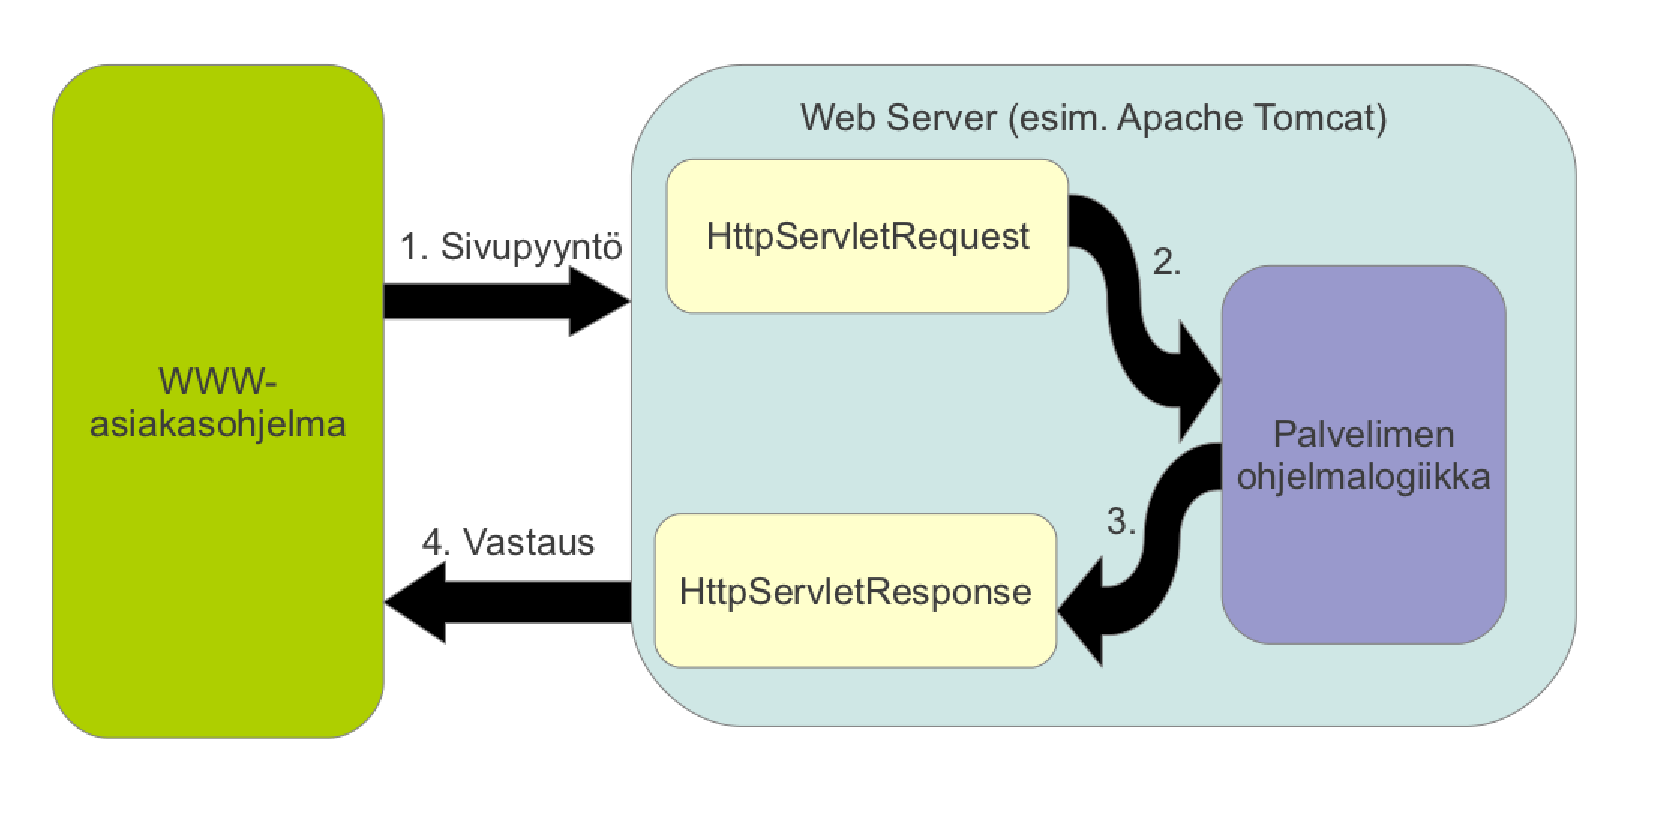
\includegraphics[width=\textwidth]{web/servlet.eps}
\caption{Kontrollin kulku Java Servlet-palvelimessa \cite{j2ee}.}%
\label{servlet}
\end{figure}
\pagebreak
Servlettien jälkeen paljon suosiota on saanut CGI:stä kehittynyt FastCGI-protokolla, joka korjaa CGI:ssä havaittuja puutteita \cite{fastcgi}. FastCGI-palvelin ei käynnistä jokaista pyyntöä kohti uutta palvelinprosessia, vaan pyynnöt lähetetään ja vas\-taan\-o\-te\-taan pistokkeen (socket) avulla palvelimella pyöriville prosesseille, jotka voivat palvella montaa pyyntöä yhtä aikaa. FastCGI-ohjelmat voidaan toteuttaa myös hajautettuna eri palvelimille, jolloin pyyntöjen välitykseen käytetään TCP-yhteyttä. FastCGI:tä voidaan käyttää minkä tahansa ohjelmointikielen kanssa, joka tukee pistokkeiden käyttöä. Näin ollen se on varteenotettava tekniikka web-sovellusten toteuttamiseen, koska ohjelmointikieli ei ole rajattu vain Javaan, vaan käytössä on useiden muiden kielten kirjo (esimerkiksi PHP, Python ja Ruby) \cite{fastcgi}.

Tiivistetysti web-sovellusten historiasta voidaan sanoa, että yksittäisistä palvelinprosesseista on kehittynyt itsenäisiä ohjelmia, joita suoritetaan jatkuvasti palvelimella. Ohjelmat saavat kontrollin joko laajentamalla web-pal\-ve\-li\-men toimintaa (Servlet, WEBrick yms) tai pistokkeiden avulla (FastCGI). Web-so\-vel\-luk\-set tuottavat käyttäjän syötteen ja web-sovelluksen sen hetkisen tilan mukaan käyttäjälle dynaamisen HTML-muotoisen sivun. Web-sovellusten kehittyessä myös niiden arkkitehtuuri on muuttunut. Web-sovellusten arkkitehtuuria käsitellään seuraavassa alaluvussa.
\subsection{Tietoturva}
Palveluiden turvallisuus koostuu kolmesta tekijästä: tunnistautumisesta (authentication), pääsynvalvonnasta (access control) ja auditoinnista (audit) \cite{sandhu}. Tunnistautumisessa käyttäjän identiteetti varmistetaan, esimerkiksi käyttäjätunnuksen ja salasanan avulla. Tämän jälkeen pääsynvalvonta tarkistaa onko kyseisellä käyttäjällä oikeutta tehdä pyytämäänsä toimintoa. Auditoinnissa analysoidaan järjestelmän tuottamaa dataa, esimerkiksi lokitiedostoja, aktiivisesti ja käyttäjän pääsy järjestelmään voidaan estää, jos luvatonta käyttöä esiintyy \cite{sandhu}.

Tämän tutkimuksen painopiste on käyttäjän tunnistautumisessa ja osittain myös pääsynvalvonnassa, auditointi ei kuulu tutkimuksen aihepiiriin. Tutkimuksessa käytetään termiä pääsynvalvonta sen suppeassa merkityksessä, toisinaan kirjallisuudessa pääsynvalvontaa pidetään kattoterminä, joka pitää sisällään tunnistautumisen, valtuutuksen (authorization) ja auditoinnin [TODO: joku lähde, jossa näin on].


\section{Tunnistautuminen ja pääsynhallinta}
Miten tunnistetaan perinteisesti?

Käyttäjädatan tallennus
- passwd (ts tiedosto levyllä tms)
- tietokanta
- AD-kannat (LDAP)

---> käyttäjän datan abstraktoinnin tarve, ehkä mainita, että käyttäjädatan backendejä voi käytännössä olla monta erilaista. Esim. LDAP:n rinnalla tietokannat.

Pituus n. 5 sivua.

Lähteitä:\\
A Guide to Computer Network Security \cite{authentication}\\
Authentication in distributed systems: theory and practice \cite{lampson}

LDAP:

Howes, T. A., The Lightweight Directory Access Protocol: X.500 Lite. CITI
Technical Report 95–8, University of Michigan, 1995. \cite{howes} \\
rfc:t 4510-4513 (ainakin 4513 "Authentication Methods and Security Mechanisms" kiinnostaa)

-----------------------------------------------------------------------------------------------------------

Tunnistautumiseen liittyvien käsitteiden läpikäynti ennen protokollien yksityiskohtaista esittelyä auttaa tunnistautumiseen liittyvien periaatteiden hahmottamista. Käsitteet ovat yleisluontoisia ja eivätkä kosketa vain tiettyjä protokollaa. Protokollien yhteydessä käytetään käsitteitä asiakasohjelma, tunnistautumispalvelu, suojattu resurssi, valtuutustieto (credentials), valtuutusavain (authorization code) ja pääsyvaltuutus (access token) \cite{nisti}.

Asiakasohjelmalla tarkoitetaan web-palvelun käyttäjän pääteohjelmaa, jolla hän kirjautuu web-palveluun käyttäen keskitettyä tunnistautumispalvelua. Käytännössä asiakasohjelma on web-palvelun tapauksessa käyttäjän WWW-selain, joka pystyy tekemään uudelleenohjauksia sivustolta toiselle. Uudelleenohjaus on HTTP-protokollan perustoiminnallisuutta, joten mikä tahansa HTTP/1.1-standardin WWW-selain käy asiakasohjelmaksi \cite{rfc2616}.

Tunnistautumispalvelu on web-palvelu, johon käyttäjä ohjataan tekemään tunnistautuminen. Onnistuneen tunnistautumisen jälkeen tunnistautumispalvelu ohjaa asi\-a\-kas\-oh\-jel\-man takaisin tunnistautumista pyytäneen palvelun määrittelemään osoitteeseen \cite{nisti}. Avoimen Internetin puolella tunnistautumispalvelu voi olla esimerkiksi Facebook tai LinkedIn.

Tunnistautumisprotokollien yhteydessä suojatulla resurssilla tarkoitetaan resurssia, jonka käyttö vaatii tunnistautumisen ja käyttöoikeuden. Yleisessä tapauksessa suojatulla resurssilla tarkoitetaan yksittäistä resurssia (käyttäjän valokuvaa), johon halutaan asettaa pääsyrajoituksia \cite{nisti}. Tämän tutkielman puitteissa suojatulla resurssilla tarkoitetaan tunnistautumista vaativaa web-palvelua.

Valtuutustieto koostuu yksilöivästä tunnisteesta ja siihen liittyvästä salaisesta avaimesta. Tämän tutkielman puitteissa valtuutustiedolla tarkoitetaan käyttäjän tunnusta ja salasanaa.

Kirjauduttuaan sisään tunnistautumispalvelimelle, käyttäjä saa valtuutusavaimen, jonka hän lähettää eteenpäin suojatun resurssin omistajalle. Valtuutusavain ei pidä sisällään käyttäjän valtuutustietoja, vaan ainoastaan tunnistautumispalvelin osaa lukea sen \cite{nisti}. Saatuaan valtuutusavaimen käyttäjältä voi suojatun resurssin omistaja hakea pääsyvaltuuden käyttäjän tietoihin tunnistautumispalvelusta.

Pääsyvaltuutus on tunnistautumispalvelimelta saatava yksilöivä tunniste, jonka avulla suojatun resurssin omistaja voi pyytää käyttäjän tiedot tunnistautumispalvelulta. Pääsyvaltuutus on voimassa tietyn ajan, jonka jälkeen se täytyy uusia tunnistautumispalvelimella \cite{nisti}. Pääsyvaltuutusta voidaan käyttää myös tunnistautumispalvelusta erillään olevien resurssien valtuuttamiseen. Esimerkiksi web-sovellus voi hakea tunnistautumispalvelulta pääsyvaltuuden, jolla hän hakee valokuvia valokuvien jakopalvelusta \cite{facebook}.
\subsection{Ympäristön kuvaus}
Lähteet:\\
- inside the identity management game \cite{inside_the_identity_management_game}\\
- Decentralization: The Future of Online Social Networking \cite{decentralisations}

Tyypillisesti web-palvelun toimintakenttä on Internet, jossa palvelut toimivat itsenäisesti. Näiden palveluiden välinen integraatio on kasvussa ja palveluiden kesken halutaan jakaa tietoa, jolloin niiden täytyy pystyä identifioimaan käyttäjä keskenään. Yleisen identeettitarjoajan rakentaminen Internettiin on tutkimuksen alla ja OpenID ja mitä näitä nyt on. 

Usein ei ole tarpeen tehdä palveluista julkisia, vaan käyttöoikeus niihin voidaan rajata tietylle osajoukolle kaikista Internetin käyttäjistä. Tällaisia osajoukkoja voi olla esimerkiksi yrityksen työntekijät, joilla on pääsy intranet-palveluihin tai tietyn sivuston käyttäjät, joilla on pääsy sivuston palveluihin. Tällöin voi olla järkevää eriyttää käyttäjähallinta omaksi palveluksi ja keskittää osapalveluiden tunnistautuminen siihen. Tämän tutkielman pääpaino on tunnetulle osajoukolle, esimerkiksi yrityksen työntekijöille, suunnatuissa palveluissa.

Tutkielmassa pyritään selvittämään kuinka yritys voi rakentaa keskitetyn tunnistautumispalvelun valmiin käyttäjädatan päälle. Lähtökohtaisesti tunnistautumista vaativat palvelut ovat web-pohjaisia, mutta myös työasemalla tai puhelimella käytettävät asiakasohjelmat pyritään ottamaan huomioon.

\subsection{Järjestelmien tietoturva}
Palveluiden turvallisuus koostuu kolmesta tekijästä: tunnistautumisesta (authentication), pääsynvalvonnasta (access control) ja auditoinnista (audit) \cite{sandhu}. Tunnistautumisessa käyttäjän identiteetti varmistetaan, esimerkiksi käyttäjätunnuksen ja salasanan avulla. Tämän jälkeen pääsynvalvonta tarkistaa onko kyseisellä käyttäjällä oikeutta tehdä pyytämäänsä toimintoa. Auditoinnissa analysoidaan järjestelmän tuottamaa dataa, esimerkiksi lokitiedostoja, aktiivisesti ja käyttäjän pääsy järjestelmään voidaan estää, jos luvatonta käyttöä esiintyy \cite{sandhu}.

Tämän tutkimuksen painopiste on käyttäjän tunnistautumisessa ja osittain myös pääsynvalvonnassa, auditointi ei kuulu tutkimuksen aihepiiriin. Tutkimuksessa käytetään termiä pääsynvalvonta sen suppeassa merkityksessä, toisinaan kirjallisuudessa pääsynvalvontaa pidetään kattoterminä, joka pitää sisällään tunnistautumisen, valtuutuksen (authorization) ja auditoinnin [TODO: joku lähde, jossa näin on].

\subsection{Käyttäjädata}
Tunnistautumiseen liittyvien käsitteiden läpikäynti ennen protokollien yksityiskohtaista esittelyä auttaa tunnistautumiseen liittyvien periaatteiden hahmottamista. Käsitteet ovat yleisluontoisia ja eivätkä kosketa vain tiettyjä protokollaa. Protokollien yhteydessä käytetään käsitteitä asiakasohjelma, tunnistautumispalvelu, suojattu resurssi, valtuutustieto (credentials), valtuutusavain (authorization code) ja pääsyvaltuutus (access token) \cite{nisti}.

Asiakasohjelmalla tarkoitetaan web-palvelun käyttäjän pääteohjelmaa, jolla hän kirjautuu web-palveluun käyttäen keskitettyä tunnistautumispalvelua. Käytännössä asiakasohjelma on web-palvelun tapauksessa käyttäjän WWW-selain, joka pystyy tekemään uudelleenohjauksia sivustolta toiselle. Uudelleenohjaus on HTTP-protokollan perustoiminnallisuutta, joten mikä tahansa HTTP/1.1-standardin WWW-selain käy asiakasohjelmaksi \cite{rfc2616}.

Tunnistautumispalvelu on web-palvelu, johon käyttäjä ohjataan tekemään tunnistautuminen. Onnistuneen tunnistautumisen jälkeen tunnistautumispalvelu ohjaa asi\-a\-kas\-oh\-jel\-man takaisin tunnistautumista pyytäneen palvelun määrittelemään osoitteeseen \cite{nisti}. Avoimen Internetin puolella tunnistautumispalvelu voi olla esimerkiksi Facebook tai LinkedIn.

Tunnistautumisprotokollien yhteydessä suojatulla resurssilla tarkoitetaan resurssia, jonka käyttö vaatii tunnistautumisen ja käyttöoikeuden. Yleisessä tapauksessa suojatulla resurssilla tarkoitetaan yksittäistä resurssia (käyttäjän valokuvaa), johon halutaan asettaa pääsyrajoituksia \cite{nisti}. Tämän tutkielman puitteissa suojatulla resurssilla tarkoitetaan tunnistautumista vaativaa web-palvelua.

Valtuutustieto koostuu yksilöivästä tunnisteesta ja siihen liittyvästä salaisesta avaimesta. Tämän tutkielman puitteissa valtuutustiedolla tarkoitetaan käyttäjän tunnusta ja salasanaa.

Kirjauduttuaan sisään tunnistautumispalvelimelle, käyttäjä saa valtuutusavaimen, jonka hän lähettää eteenpäin suojatun resurssin omistajalle. Valtuutusavain ei pidä sisällään käyttäjän valtuutustietoja, vaan ainoastaan tunnistautumispalvelin osaa lukea sen \cite{nisti}. Saatuaan valtuutusavaimen käyttäjältä voi suojatun resurssin omistaja hakea pääsyvaltuuden käyttäjän tietoihin tunnistautumispalvelusta.

Pääsyvaltuutus on tunnistautumispalvelimelta saatava yksilöivä tunniste, jonka avulla suojatun resurssin omistaja voi pyytää käyttäjän tiedot tunnistautumispalvelulta. Pääsyvaltuutus on voimassa tietyn ajan, jonka jälkeen se täytyy uusia tunnistautumispalvelimella \cite{nisti}. Pääsyvaltuutusta voidaan käyttää myös tunnistautumispalvelusta erillään olevien resurssien valtuuttamiseen. Esimerkiksi web-sovellus voi hakea tunnistautumispalvelulta pääsyvaltuuden, jolla hän hakee valokuvia valokuvien jakopalvelusta \cite{facebook}.
\subsubsection{passwd}
Vanha kunnon /etc/passwd, tästä tunnistautuminen on varmaan lähtenyt käyntiin. Ikävää, kun webiin tunnistautuessa täytyy olla tunnus kyseisellä koneella ja muutenkin ei ole hyvä kun tunnukset siirtyy verkkoa pitkin.
\subsubsection{Relaatiotietokannat}
Käyttäjätietokannat, relaatiokannat lähinnä, ehkä NoSQL.
\subsubsection{LDAP}
Lähteet: Howes, T. A., The Lightweight Directory Access Protocol: X.500 Lite. CITI
Technical Report 95–8, University of Michigan, 1995. \cite{howes} \\
rfc:t 4510-4513 (ainakin 4513 "Authentication Methods and Security Mechanisms" kiinnostaa)

Lightweight Directory Access Protocol (LDAP) on X.500 OSI-standardiin perustuva hakemistopalvelu, jota käytetään yleisesti käyttäjätiedon tallennukseen [TODO: lähde]. 1990-luvulla TCP/IP-mallin syrjäytettyä OSI-mallin, myös DAP kävi vanhanaikaiseksi \cite{howes}. Korvaajaksi on noussut LDAP, josta käytetään myös nimeä X.500 Lite \cite{howes}.

LDAP:ssa asiakassovellukset (directory user agent, DUA) keskustelevat puumalliin perustuvan hakemistopalvelimen (directory system agent, DSA) kanssa käyttäen määriteltyä protokollaa (directory access protocol, DAP) \cite{howes}. Asiakassovellukset voivat hakea hakemistopalvelimesta tietoa suodattimiin (filter) perustuvalla lukuoperaatiolla. Suodattimessa voidaan määritellä raja-arvot attribuutin arvolle tai hakea avainsanoilla attribuuteista.

LDAP-tietuille voidaan määritellä pakollisten attribuuttien (esim. etu- ja sukunimi) lisäksi valinnaisia attribuutteja. Tietueet on järjestetty puuhun niiden yksilöivän nimen (distinguished name, DN) mukaan ja ne voi olla hajautettu usealle palvelimelle. Suhteellinen nimi (relative distinguished name, RDN) identifioi tietueen omalla hierarkiatasollaan.

LDAP-tietueella voi olla tunnus sekä salasana ja LDAP-palvelinta voidaan käyttää käyttäjän tunnistautumiseen [TODO: lähde, ehkä rfc4513].

TODO: lisää tekstiä

\subsubsection{Käyttäjädatan abstraktointi}
Tutkimuksen kannalta abstraktointi on oleellista, oikeastaan sillä ei ole ison kuvan kannalta merkitystä, että onko siellä taustalla tietokanta, tiedosto, ldap vai mikä.
\subsection{Yhteenveto}
Käytetään OAuthia protossa, koska OpenID:ssä kaikkea tarpeetonta mukana. SAML taas skipataan, koska...? Tätä pitäisi pohtia jossain kohtaa.

\section{Keskitetyn tunnistautumisen teknologiat}
Palveluperustaisten arkkitehtuurien myötä organisaation sisällä saattaa olla useita web-palveluita, jotka haluavat myös tunnistaa käyttäjän. Tässä luvussa pureudutaan tähän liittyvään ongelmakenttään. Vaikka web-sovellusten määrä järjestelmässä kasvaa, halutaan käyttäjien tunnistetiedot pitää keskitettynä, jotta vältytään erilaisilta tietoturva- ja synkronointiongelmilta.

Organisaatioiden sisäisissä palveluissa Facebookin tai LinkedInin kaltaisten palveluiden käyttö ei välttämättä tule kysymykseen. Intranet-järjestelmien ylläpitäjät eivät mahdollisesti halua siirtää käyttäjähallintaansa ulkopuolisen yrityksen haltuun, vaan olemassaolevia hallintajärjestelmiä halutaan käyttää. Seuraavassa luvussa käydään läpi ongelmia, joita nykyisten käyttäjähallintajärjestelmien integrointi palvelusuuntautuneisiin arkkitehtuureihin tuottaa ja esitetään ratkaisuksi keskitettyä tunnistautumispalvelua.





Tämän tutkielman kannalta tunnistamisen luotettavuus ei ole teknisiä yksityiskohdat eivät ole merkityksellisiä, vaan ne ovat tunnistautumispalvelun toteutukseen yksityiskohtia. Tunnistautumispalveluun liitetyn web-sovelluksen täytyy luottaa siihen, että käyttäjät tunnistetaan luotettavasti.




Keskitetyn tunnistautumisen tarkoituksena on tarjota palvelu, jota vasten käyttäjä voidaan tunnistaa erillisestä web-palvelusta ilman uuden identiteetin luontia. Tunnistautumispalvelun ja sitä käyttävien web-palveluiden välillä on luottamussuhde, jolloin web-palveluun ei tarvitse luoda omaa käyttäjille tunnistautumistietoja (käyttäjätunnus/salasana), vaan se voi luottaa tunnistautumispalvelun tunnistamiin käyttäjiin.

Tunnistautumispalvelulla parannetaan järjestelmien tietoturvaa ja tunnistautumisen luotettavuutta. Käyttäjät valitsevat vahvempia salasanoja palveluihin, jotka he kokeavat tärkeiksi, kuten sähköpostiin, verrattuna vähemmän tärkeisiin web-palveluihin \cite{password_habits}. Keskitetyssä palvelussa käyttäjän tunnistautumisen luotettavuutta voidaan parantaa esimerkiksi vaatimalla normaalia web-palvelua vahvempia salasanoja. Käyttäjien todennusta voidaan vahvistaa myös lisävarmistuksilla, kuten erilaisilla tunnuslukulistoilla tai puhelimen kautta tehtävällä todennuksella. Käyttäjä ei tarvitse organisaation jokaiseen järjestelmään eri tunnistautumistietoja, vaan yksi riittää koko organisaation laajuudessa.

Kääntöpuolena keskitetyssä ratkaisussa on käytetyn tunnuksen ja salasanan kalastelun käyminen houkuttelevaksi, koska sen avulla pääsee käyttäjän nimissä useaan palveluun tai jopa luomaan käyttäjän identiteetillä tunnuksia uusin palveluihin. Tästä syystä palveluun kohdistuu normaalia web-palvelua suuremmat odotukset tietoturvalle, joten käytettyjen teknologioiden täytyy olla luotettavia.

Keskitetyn ratkaisun myötä erillisten web-palveluiden ei tarvitse integroitua suoraan organisaation käyttäjähallintajärjestelmiin, vaan pelkästään tunnistautumispalvelulla on pääsy sinne. Pelko käyttäjiä koskevan datan joutumisesta vääriin käsiin vähenee, koska suoraa integraatiota ei tehdä yksittäisistä palveluista, vaan tunnistautumispalvelu toimii "palomuurina". Pahimmassa tilanteessa käyttäjädata, ja käyttäjiin liittyviä tunnistautumistieto käyttäjätunnuksineen ja salasanoineen, on kopioitu jokaiseen erilliseen web-palveluun ja palvelut eivät edes tunnistaudu käyttäjähallintajärjestelmiin. Tästä seuraa aiemmin mainittuja synkronointiongelmia esimerkiksi henkilön jättäessä organisaation.

Web-palvelun ulkopuolisen tunnistautumissivun toteuttamiseen on kehitetty useita tunnistautumisprotokollia, joilla tunnistautuminen voidaan tehdä turvalliseksi ja käyttäjälle helpoksi [TODO: lähde]. Tunnistautumisprotokollat ovat käytössä avoimen Internetin puolella, esimerkiksi Facebookilla ja Googlella on ollut merkittävä rooli näiden protokollien syntyhistoriassa [TODO: lähde]. Protokollia käsitellään tarkemmin seuraavassa luvussa.
\section{Toteutus}
Tunnistautumiseen liittyvien käsitteiden läpikäynti ennen protokollien yksityiskohtaista esittelyä auttaa tunnistautumiseen liittyvien periaatteiden hahmottamista. Käsitteet ovat yleisluontoisia ja eivätkä kosketa vain tiettyjä protokollaa. Protokollien yhteydessä käytetään käsitteitä asiakasohjelma, tunnistautumispalvelu, suojattu resurssi, valtuutustieto (credentials), valtuutusavain (authorization code) ja pääsyvaltuutus (access token) \cite{nisti}.

Asiakasohjelmalla tarkoitetaan web-palvelun käyttäjän pääteohjelmaa, jolla hän kirjautuu web-palveluun käyttäen keskitettyä tunnistautumispalvelua. Käytännössä asiakasohjelma on web-palvelun tapauksessa käyttäjän WWW-selain, joka pystyy tekemään uudelleenohjauksia sivustolta toiselle. Uudelleenohjaus on HTTP-protokollan perustoiminnallisuutta, joten mikä tahansa HTTP/1.1-standardin WWW-selain käy asiakasohjelmaksi \cite{rfc2616}.

Tunnistautumispalvelu on web-palvelu, johon käyttäjä ohjataan tekemään tunnistautuminen. Onnistuneen tunnistautumisen jälkeen tunnistautumispalvelu ohjaa asi\-a\-kas\-oh\-jel\-man takaisin tunnistautumista pyytäneen palvelun määrittelemään osoitteeseen \cite{nisti}. Avoimen Internetin puolella tunnistautumispalvelu voi olla esimerkiksi Facebook tai LinkedIn.

Tunnistautumisprotokollien yhteydessä suojatulla resurssilla tarkoitetaan resurssia, jonka käyttö vaatii tunnistautumisen ja käyttöoikeuden. Yleisessä tapauksessa suojatulla resurssilla tarkoitetaan yksittäistä resurssia (käyttäjän valokuvaa), johon halutaan asettaa pääsyrajoituksia \cite{nisti}. Tämän tutkielman puitteissa suojatulla resurssilla tarkoitetaan tunnistautumista vaativaa web-palvelua.

Valtuutustieto koostuu yksilöivästä tunnisteesta ja siihen liittyvästä salaisesta avaimesta. Tämän tutkielman puitteissa valtuutustiedolla tarkoitetaan käyttäjän tunnusta ja salasanaa.

Kirjauduttuaan sisään tunnistautumispalvelimelle, käyttäjä saa valtuutusavaimen, jonka hän lähettää eteenpäin suojatun resurssin omistajalle. Valtuutusavain ei pidä sisällään käyttäjän valtuutustietoja, vaan ainoastaan tunnistautumispalvelin osaa lukea sen \cite{nisti}. Saatuaan valtuutusavaimen käyttäjältä voi suojatun resurssin omistaja hakea pääsyvaltuuden käyttäjän tietoihin tunnistautumispalvelusta.

Pääsyvaltuutus on tunnistautumispalvelimelta saatava yksilöivä tunniste, jonka avulla suojatun resurssin omistaja voi pyytää käyttäjän tiedot tunnistautumispalvelulta. Pääsyvaltuutus on voimassa tietyn ajan, jonka jälkeen se täytyy uusia tunnistautumispalvelimella \cite{nisti}. Pääsyvaltuutusta voidaan käyttää myös tunnistautumispalvelusta erillään olevien resurssien valtuuttamiseen. Esimerkiksi web-sovellus voi hakea tunnistautumispalvelulta pääsyvaltuuden, jolla hän hakee valokuvia valokuvien jakopalvelusta \cite{facebook}.
\subsection{Järjestelmän nykytila}
Sikteeri on vuosien varrella paisunut yleiseksi toiminnanohjausjärjestelmäksi, jonka arkkitehtuuria kehittäjät haluaisivat viedä palvelusuuntautuneiden arkkitehtuurien suuntaan, jotta yksittäisten palveluiden kehittäminen olisi kevyempää. Jotta Sikteerin ulkopuolisten web-palveluiden kehittäminen on mahdollista, täytyy erillisillä palveluilla olla tapa tunnistaa käyttäjä. Varsinainen käyttäjähallinta on tällä hetkellä Sikteerin ulkopuolisessa LDAP-tietokannassa, jota vasten Sikteeri tunnistaa käyttäjät. Nykyistä LDAP-tietokantaa halutaan käyttää myös jatkossa keskitetyssä tunnistautumispalvelussa, mutta Sikteerin (tai muun vastaavan palvelun) ei tarvitse päästä suoraan LDAP-kantaan käsiksi.

Sikteeri on Kapsi ry:n laskutuksen ja jäsenhallinnan tarpeisiin kehitetty web-palvelu. Sikteeriin on pääsy Kapsi ry:n hallituksella, ylläpidolla ja ryhmään laskutus kuuluvilla jäsenillä. Lisäksi yhdistyksellä on käytössään erillinen komentorivityökalu, nimeltä admtool, jolla voidaan tehdä erilaisia ylläpitotehtäviä.

Sekä Sikteeri että admtool käyttävät ulkoisena komponenttina LDAP-käyt\-tä\-jä\-hal\-lin\-taa, josta tarkistetaan onko käyttäjällä oikeuksia käyttää kyseisiä palveluita. Nykyinen arkkitehtuuri on kuvattu kuvassa \ref{kapsi_nykyinen}. Kuvaan on lisätty myös suunnitteilla oleva käyttäjien palvelunhallinta, jota kautta jäsenet voisivat lisätä itselleen jäsenmaksuun kuuluvia palveluita, kuten sähköpostialiaksia ja domaineja. Myös käyttäjien palvelunhallinnan tarvitsee tunnistaa käyttäjät, joten nykyisessä arkkitehtuurissa myös sen täytyy integroitua LDAP-käyttäjänhallintaan.

\begin{figure}[h]
\centering
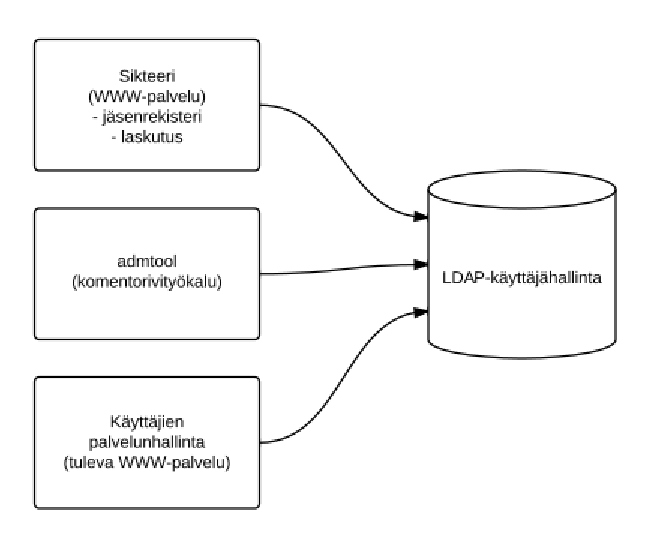
\includegraphics[width=.7\textwidth]{toteutus/kapsi_nykyinen.eps}
\caption{Kapsin jäsenhallintapalveluiden arkkitehtuuri.}%
\label{kapsi_nykyinen}
\end{figure}

Nykyisellään Sikteeri käyttää Django-ohjelmistokehyksen tarjoamaa väliohjelmistoa tunnistautumiseen. Django.contrib.auth-niminen väliohjelmisto tarjoaa hyvät laajentamismahdollisuudet \cite{django_auth}. Siinä on mahdollista määritellä eri taustajärjestelmiä (backend), joita käytetään tunnistautumisessa. Sikteeri käyttää tunnistautumiseen Djangon tarjoamaa ModelBackend-taustajärjestelmää, joka mahdollistaa käyttäjän tunnistautumisen vertaamalla käyttäjän syöttämää käyttäjätunnusta ja salasanaa tietokantaan tallennettuihin käyttäjiin \cite{django_auth}. Jos oikealla tunnus/salasana-parilla oleva käyttäjä löytyy, palautetaan se sovellustasolle.
\subsection{Järjestelmän muutostarve}
Tunnistautumiseen liittyvien käsitteiden läpikäynti ennen protokollien yksityiskohtaista esittelyä auttaa tunnistautumiseen liittyvien periaatteiden hahmottamista. Käsitteet ovat yleisluontoisia ja eivätkä kosketa vain tiettyjä protokollaa. Protokollien yhteydessä käytetään käsitteitä asiakasohjelma, tunnistautumispalvelu, suojattu resurssi, valtuutustieto (credentials), valtuutusavain (authorization code) ja pääsyvaltuutus (access token) \cite{nisti}.

Asiakasohjelmalla tarkoitetaan web-palvelun käyttäjän pääteohjelmaa, jolla hän kirjautuu web-palveluun käyttäen keskitettyä tunnistautumispalvelua. Käytännössä asiakasohjelma on web-palvelun tapauksessa käyttäjän WWW-selain, joka pystyy tekemään uudelleenohjauksia sivustolta toiselle. Uudelleenohjaus on HTTP-protokollan perustoiminnallisuutta, joten mikä tahansa HTTP/1.1-standardin WWW-selain käy asiakasohjelmaksi \cite{rfc2616}.

Tunnistautumispalvelu on web-palvelu, johon käyttäjä ohjataan tekemään tunnistautuminen. Onnistuneen tunnistautumisen jälkeen tunnistautumispalvelu ohjaa asi\-a\-kas\-oh\-jel\-man takaisin tunnistautumista pyytäneen palvelun määrittelemään osoitteeseen \cite{nisti}. Avoimen Internetin puolella tunnistautumispalvelu voi olla esimerkiksi Facebook tai LinkedIn.

Tunnistautumisprotokollien yhteydessä suojatulla resurssilla tarkoitetaan resurssia, jonka käyttö vaatii tunnistautumisen ja käyttöoikeuden. Yleisessä tapauksessa suojatulla resurssilla tarkoitetaan yksittäistä resurssia (käyttäjän valokuvaa), johon halutaan asettaa pääsyrajoituksia \cite{nisti}. Tämän tutkielman puitteissa suojatulla resurssilla tarkoitetaan tunnistautumista vaativaa web-palvelua.

Valtuutustieto koostuu yksilöivästä tunnisteesta ja siihen liittyvästä salaisesta avaimesta. Tämän tutkielman puitteissa valtuutustiedolla tarkoitetaan käyttäjän tunnusta ja salasanaa.

Kirjauduttuaan sisään tunnistautumispalvelimelle, käyttäjä saa valtuutusavaimen, jonka hän lähettää eteenpäin suojatun resurssin omistajalle. Valtuutusavain ei pidä sisällään käyttäjän valtuutustietoja, vaan ainoastaan tunnistautumispalvelin osaa lukea sen \cite{nisti}. Saatuaan valtuutusavaimen käyttäjältä voi suojatun resurssin omistaja hakea pääsyvaltuuden käyttäjän tietoihin tunnistautumispalvelusta.

Pääsyvaltuutus on tunnistautumispalvelimelta saatava yksilöivä tunniste, jonka avulla suojatun resurssin omistaja voi pyytää käyttäjän tiedot tunnistautumispalvelulta. Pääsyvaltuutus on voimassa tietyn ajan, jonka jälkeen se täytyy uusia tunnistautumispalvelimella \cite{nisti}. Pääsyvaltuutusta voidaan käyttää myös tunnistautumispalvelusta erillään olevien resurssien valtuuttamiseen. Esimerkiksi web-sovellus voi hakea tunnistautumispalvelulta pääsyvaltuuden, jolla hän hakee valokuvia valokuvien jakopalvelusta \cite{facebook}.
Nykyinen toimintaympäristö, sekä Kapsin omat käytännöt, asettavat vaatimuksia ja reunaehtoja toteutukselle. Enimmäkseen nämä vaatimukset johtuvat käytetystä Python-kielestä ja halusta tukea avointa ohjelmistokehitystä.

Järjestelmän ylläpidon helpottamiseksi uudet komponentit halutaan toteuttaa Pythonilla, koska Sikteeri ja admtool on toteutettu sillä. Toteutuksessa halutaan käyttää mahdollisimman paljon avoimen lähdekoodin alaista koodia, joten tunnistautumispalvelussa käytetystä protokollasta täytyy olla Python-kielellä toteutettu ratkaisu. Toisaalta järjestelmän sisällä ei haluta sulkea muiden ohjelmointikielten tai -kehysten käyttöä pois, joten pelkästään Python-kielinen ratkaisu ei riitä, vaan standardejen täytyy olla avoimia ja käytettävissä myös Javan web-kehyksillä tai esimerkiksi Ruby on Rails -ohjelmointikehyksellä.

Tunnistautumispalvelun täytyy tukea myös komentorivityökaluja, kuten nykyistä admtoolia. Tällöin pelkkä käyttäjäagentti-pohjainen tunnistamismenetelmä ei riitä, vaan tunnistamisen täytyy olla mahdollista ilman selainta.

Käyttäjän tunnistaminen ei riitä yksinään, vaan tunnistautumispalvelun täytyy tukea myös käyttäjään liittyvien parametrien välitystä. Tämä on tärkeää, koska järjestelmässä on eri tasoisia käyttäjiä (hallitus, toimihenkilöt ja ylläpito) ja tunnistautumispalvelua käyttävän sovelluksen täytyy tietää, mihin käyttäjäryhmään tunnistettu käyttäjä kuuluu. Myös muita käyttäjään liittyviä attribuutteja, kuten sähköpostiosoitetta tai puhelinnumeroa, tarvitaan sovelluksissa.

Valitun tunnistautumisprotokollan täytyy olla sellainen, että nykyisten sovellusten muuttaminen käyttämään uutta tunnistautumismekanismia on helppoa. Tämä tarkoittaa, että koodiin täytyy tehdä mahdollisimman vähän muutoksia. Nykyisissä toteutuksissa on käytetty Djangon vakio-tunnistautumismekanismia, joka toimii väliohjelmakerroksessa. Käytettävästä tunnistautumisprotokollasta olisi hyvä olla valmis avoimen lähdekoodin Django-valiohjelmatoteutus jo olemassa.
\subsection{Järjestelmän uusi arkkitehtuuri}
Palveluun tehtävät muutokset jakautuvat kahteen osaan: Sikteerin muutoksiin ja uuteen keskitettyyn tunnistautumispalveluun. Muutoksien jälkeen Sikteeri ei käytä omaa käyttäjähallintaa tunnistamiseen, vaan tunnistaminen tapahtuu keskitetyssä tunnistautumispalvelussa, joka käyttää hyväkseen Kapsin LDAP-käyttäjähallintaa.

Seuraavissa aliluvuissa käydään ensin läpi Sikteeriin vaadittavia muutoksia, jotta sitä voidaan käyttää yhdessä ulkoisen tunnistautumispalvelun kanssa. Tämän jälkeen määritellään uuden tunnistautumispalvelun toiminta ja hahmotellaan sen arkkitehtuuri.

\subsubsection{Sikteeri}
Nykyisellään Sikteeri käyttää Django-ohjelmistokehyksen tarjoamaa väliohjelmistoa tunnistautumiseen. Django.contrib.auth-niminen väliohjelmisto tarjoaa hyvät laajentamismahdollisuudet \cite{django_auth}. Siinä on mahdollista määritellä eri taustajärjestelmiä (backend), joita käytetään tunnistautumisessa. Sikteeri käyttää tunnistautumiseen Djangon tarjoamaa ModelBackend-taustajärjestelmää, joka mahdollistaa käyttäjän tunnistautumisen vertaamalla käyttäjän syöttämää käyttäjätunnusta ja salasanaa tietokantaan tallennettuihin käyttäjiin \cite{django_auth}. Jos oikealla tunnus/salasana-parilla oleva käyttäjä löytyy, palautetaan se sovellustasolle.

Ulkoista tunnistautumispalvelua käytettäessä ModelBackend korvataan uudella taustajärjestelmällä. Taustajärjestelmän toiminta on esitetty kuvassa \ref{auth_kapsi_fi_flow}. Sikteeri siis ohjaa käyttäjän tunnistautumispalveluun, josta lähetetään onnistuneen tunnistautumisen jälkeen valtuutusavain Sikteerille. Valtuutusavaimella Sikteerin väliohjelmisto hakee käyttäjän tiedot jälleen tunnistautumispalvelusta ja etsii tietokannastaan käyttäjätunnusta vastaavan käyttäjän tiedot.

Uusitussa Sikteerissä käyttäjät tallennetaan edelleen entiseen tapaan sen omaan tietokantaan. Käyttäjätunnus yksilöi käyttäjän Kapsin järjestelmissä, joten se täytyy olla tietokannassa käyttäjän tunnistamista varten. Sen sijaan Sikteerin tietokannasta voi poistaa salasana-sarakkeen, sillä paikallista salasanaa ei käytetä enää jatkossa. Käyttäjien tiedot tallennetaan Sikteeriin, koska käyttäjällä on vain Sikteeriin liittyviä attribuutteja, joita ei haluta tallettaa käyttäjähallintaan.

Sikteerin käyttäjän näkökulmasta järjestelmän toiminta ei poikkea merkittävästi vanhasta. Sikteerin tarjoaman kirjautumislomakkeen sijaan käyttäjä ohjataan tekemään tunnistautuminen ulkoiselle palvelimelle.
\subsubsection{Tunnistautumispalvelu auth.kapsi.fi}
Uuteen arkkitehtuuriin liittyvä tunnistautumispalvelu (auth.kapsi.fi) tarjoaa kaksi erillistä rajapintaa, joista ensimäinen on käyttäjälle näkyvä kirjautumissivu. Toisen rajapinnan kautta web-palvelut voivat hakea käyttäjän tiedot valtuutusavaimen avulla. Tunnistautumispalvelun täytyy tarjota molemmat rajapinnat, koska siinä on päätetty käyttää OAuth-protokollaa.

Tunnistautumispalvelu on yhteydessä Kapsin käyttäjähallintaan, joka on LDAP-tietokannassa. Käyttäjähallinnan ja tunnistautumispalvelun väliseen kommunikointiin käytetään LDAPBack\-end-taustajärjestelmää, jonka toimintaperiaate on samankaltainen kuin Sikteerissä käytetyssä ModelBackend-taustajärjestelmästä. Jatkossa järjestelmän salasana on tallennettu vain LDAP-tietokantaan ja sitä ei kopioida yksittäisiin palveluihin, kuten tähän asti.

Jotta tunnistautumispalvelu toimisi halutulla tavalla, täytyy sitä käyttäville web-palveluille (esim. Sikteeri) määritellä palvelun tunnus ja yhteinen jaettu salainen avain \cite{oauth2_0}. Näiden avulla voidaan varmistua siitä, että tunnistautumispyyntö tulee varmasti hyväksyttävästä lähteestä ja käyttäjä ei pysty väärentämään valtuutusavainta. Tällä suojataan käyttäjän tietoja ja estetään niiden joutumisen vääriin käsiin. Myös auditointi on mahdollista, kun tunnistautumispalvelun lokitiedostoista voidaan katsoa mihin palveluihin ja koska käyttäjä on kirjautunut.

Nykyään pääsynvalvonta toteutetaan Sikteerissä vertaamalla tunnistautumispalvelulta saatavaa käyttäjätunnusta Sikteerin tietokannassa määriteltyihin tunnuksiin, joilla on oikeus käyttää palvelua. Tulevaisuudessa tunnistautumispalvelun voisi palauttaa käyttäjän tietojen mukana listan käyttäjän oikeuksista, joiden avulla web-palvelu voi päättää, onko käyttäjällä oikeus päästä järjestelmään. Pääsynvalvonta voidaan toteuttaa myös tunnistautumispalvelussa, jolloin se paluttaa Sikteerille käyttäjän tiedot vain, jos käyttäjällä on oikeus päästä järjestelmään. Nykytoteutuksessa tiedot palautetaan joka tapauksessa ja Sikteeri tekee päätöksen, onko käyttö sallittu. Arkkitehtuurin pohditaan seuraavassa luvussa, jossa myös arvioidaan täyttääkö uusi arkkitehtuuri sille asetetut vaatimukset.
\section{Toteutuksen evaluaatio}
Otsikoita vois vielä katsoa kohdalleen.

\subsection{Edut nykyiseen toteutukseen nähden}
Tunnistautumiseen liittyvien käsitteiden läpikäynti ennen protokollien yksityiskohtaista esittelyä auttaa tunnistautumiseen liittyvien periaatteiden hahmottamista. Käsitteet ovat yleisluontoisia ja eivätkä kosketa vain tiettyjä protokollaa. Protokollien yhteydessä käytetään käsitteitä asiakasohjelma, tunnistautumispalvelu, suojattu resurssi, valtuutustieto (credentials), valtuutusavain (authorization code) ja pääsyvaltuutus (access token) \cite{nisti}.

Asiakasohjelmalla tarkoitetaan web-palvelun käyttäjän pääteohjelmaa, jolla hän kirjautuu web-palveluun käyttäen keskitettyä tunnistautumispalvelua. Käytännössä asiakasohjelma on web-palvelun tapauksessa käyttäjän WWW-selain, joka pystyy tekemään uudelleenohjauksia sivustolta toiselle. Uudelleenohjaus on HTTP-protokollan perustoiminnallisuutta, joten mikä tahansa HTTP/1.1-standardin WWW-selain käy asiakasohjelmaksi \cite{rfc2616}.

Tunnistautumispalvelu on web-palvelu, johon käyttäjä ohjataan tekemään tunnistautuminen. Onnistuneen tunnistautumisen jälkeen tunnistautumispalvelu ohjaa asi\-a\-kas\-oh\-jel\-man takaisin tunnistautumista pyytäneen palvelun määrittelemään osoitteeseen \cite{nisti}. Avoimen Internetin puolella tunnistautumispalvelu voi olla esimerkiksi Facebook tai LinkedIn.

Tunnistautumisprotokollien yhteydessä suojatulla resurssilla tarkoitetaan resurssia, jonka käyttö vaatii tunnistautumisen ja käyttöoikeuden. Yleisessä tapauksessa suojatulla resurssilla tarkoitetaan yksittäistä resurssia (käyttäjän valokuvaa), johon halutaan asettaa pääsyrajoituksia \cite{nisti}. Tämän tutkielman puitteissa suojatulla resurssilla tarkoitetaan tunnistautumista vaativaa web-palvelua.

Valtuutustieto koostuu yksilöivästä tunnisteesta ja siihen liittyvästä salaisesta avaimesta. Tämän tutkielman puitteissa valtuutustiedolla tarkoitetaan käyttäjän tunnusta ja salasanaa.

Kirjauduttuaan sisään tunnistautumispalvelimelle, käyttäjä saa valtuutusavaimen, jonka hän lähettää eteenpäin suojatun resurssin omistajalle. Valtuutusavain ei pidä sisällään käyttäjän valtuutustietoja, vaan ainoastaan tunnistautumispalvelin osaa lukea sen \cite{nisti}. Saatuaan valtuutusavaimen käyttäjältä voi suojatun resurssin omistaja hakea pääsyvaltuuden käyttäjän tietoihin tunnistautumispalvelusta.

Pääsyvaltuutus on tunnistautumispalvelimelta saatava yksilöivä tunniste, jonka avulla suojatun resurssin omistaja voi pyytää käyttäjän tiedot tunnistautumispalvelulta. Pääsyvaltuutus on voimassa tietyn ajan, jonka jälkeen se täytyy uusia tunnistautumispalvelimella \cite{nisti}. Pääsyvaltuutusta voidaan käyttää myös tunnistautumispalvelusta erillään olevien resurssien valtuuttamiseen. Esimerkiksi web-sovellus voi hakea tunnistautumispalvelulta pääsyvaltuuden, jolla hän hakee valokuvia valokuvien jakopalvelusta \cite{facebook}.

\subsubsection{Ylläpito}
Kapsi ryn ylläpidon näkökulmasta suurin etu on järjestelmän yleisen tietoturvan parantuminen. Käyttäjähallintaa voidaan pitää kriittisenä komponenttina ja kun vain tunnistautumispalvelu integroituu siihen, paranee järjestelmän yleinen tietoturva \cite{arkkitehtuurit}. Lisäksi käyttäjien tunnistautumistietoja ei enää tarvitse kopioida sovelluksien käyttöön, koska käyttäjät tunnistetaan OAuth-protokollan avulla \cite{oauth2_0}. Riski salasanatiivisteiden tms tunnistetietojen leviämiseen järjestelmän ulkopuolelle pienenee, koska kriittinen käyttäjädata on tallennettu vain yhteen paikkaan.

Muutosten tekeminen tunnistautumisen tekniikoihin helpottuu, kun käyttäjät tunnistautuvat vain yhden palvelun kautta. Esimerkiksi Googlen palveluita käytettäessä on mahdollista käyttää niin kutsuttua kahden tekijän tunnistautumista (two factor authentication) \cite{google_two_factor}. Tällöin tunnuksen ja salasanan lisäksi palvelu pyytää syöttämään tunnistuskoodin, joka lähetetään käyttäjän matkapuhelimeen. Tällöin tiedetään, että tunnuksen ja salasanan lisäksi käyttäjällä on pääsy myös järjestelmään rekisteröimäänsä matkapuhelimeen, joten tunnistusta voidaan pitää normaalia tunnistautumista tehokkaampana \cite{}. Tällaisen tunnistautumista vahvistavan toimenpiteen tuominen Kapsin järjestelmiin on mahdollista ilman, että web-palveluiden koodia tarvitsee muuttaa, kun esimerkkiarkkitehtuurin mukainen tunnistautumispalvelu on käytössä.

\subsubsection{Web-palveluiden kehittäjät}
Kehittäjän näkökulmasta suurin etu uudesta arkkitehtuurista on web-sovellusten entistä helpompi liitettävyys osaksi Kapsin järjestelmää. Web-sovelluksen kehittäjän ei tarvitse rakentaa sovellukseensa käyttäjähallintaa, vaan se on käytettävissä ulkoisena palveluna. Sovelluksen ohjelmoijan ei tarvitse myöskään huolehtia käyttäjätietokannan synkronoinnista, vaan käyttäjätiedot ovat aina ajan tasalla.

Kun palveluiden ja tunnistautumispalvelun välillä käytetään luotettavaa protokollaa, voivat ylläpitäjät sallia web-sovellusten pääsyn tunnistautumispalveluun, vaikka eivät tuntisikaan web-sovelluksen toimintaa. Esimerkiksi Facebook hyödyntää tätä ominaisuutta tarjoamalla käyttäjiensä toteuttamille web-sovelluksille mahdollisuuden käyttää Facebook-tunnuksia tunnistautumiseen. Samaan tapaan Kapsin jäsenet voisivat tuottaa omia palveluita muiden jäsenten käyttöön. Uuden arkkitehtuurin myötä myös muut kuin järjestelmän ylläpitäjät voivat Facebookin tapaan tehdä omia palveluita Kapsin jäsenille.

\subsubsection{Jäsenet}
Sikteerin käyttäjän näkökulmasta uuden järjestelmän toiminta ei poikkea merkittävästi vanhasta ja uuden arkkitehtuurin tuomat edut ovat lähinnä epäsuoria. Sikteerin tarjoaman kirjautumislomakkeen sijaan käyttäjä ohjataan tekemään tunnistautuminen ulkoiselle palvelimelle. Tämä parantaa järjestelmän tietoturvaa ja vähentää riskiä käyttäjän tietojen vuotamisesta ulkopuoliselle taholle.

Arkkitehtuurin muutoksen jälkeen Sikteerissä ei käytetä enää erillistä salasanaa, vaan muutoksen jälkeen sama salasana on käytössä kaikkialla. Myös mahdollisiin tuleviin palveluihin ei tarvita enää erillistä salasanaa, vaan samalla salasanalla voi kirjautua kaikkiin Kapsin palveluihin. Tällainen uusi palvelu voisi olla esimerkiksi web-sovellus, jonka kautta käyttäjä voi lisätä jäsenetuihin kuuluvia sähköpostitunnuksia. Myös mahdollisuus saada käyttöön uusia web-sovelluksia on epäsuora etu käyttäjälle.

Jos arkkitehtuuri laajennetaan mahdollistamaan kertakirjautuminen, myös käyttäjät hyötyvät entistä enemmän, koska jokaiseen järjestelmän palveluun ei tarvitse enää kirjautua erikseen. Tämä vaatii jonkun verran laajennuksia arkkitehtuuriin, ja niitä käsitellään tarkemmin aliluvussa 6.3.

\subsection{Ongelmat ja rajoitukset}
Kun Kapsin tietojärjestelmissä siirrytään keskitetyn tunnistautumispalvelun käyttöön, joudutaan tunnistautumista vaativat web-sovellukset muuttaa käyttämään uutta tunnistautumisjärjestelmää. Ohjelman toiminnan kannalta tällä ei saavuteta varsinaisesti mitään hyötyä, joten kyseessä on epätoivottu heijastusvaikutus (ripple effect). Heijastusvaikutuksella tarkoitetaan muutoksia, joita joudutaan tekemään ohjelmaan, joita alkuperäiset muutokset eivät suoraan koske \cite{arkkitehtuurit}. Toisaalta ratkaisulla vähennetään heijastusvaikutuksia tulevaisuudessa, kun web-sovelluksen ja tunnistautumisen välinen vahva riippuvuussuhde puretaan \cite{arkkitehtuurit}. Tällöin esimerkiksi kaksivaiheisen kirjautumisen toteuttaminen järjestelmään ei vaadi muutoksia kirjautumista käyttäviin web-sovelluksiin.

Tunnistautumispalvelu on erittäin kriittinen komponentti arkkitehtuurissa ja sen kaatuminen estää web-sovellusten täysipainoisen käytön, koska käyttäjien kirjautuminen ei ole mahdollista. Web-sovellukset tulevat siis riippuvaiseksi ulkoisesta (tunnistautumis)palvelusta, jolloin sovelluksen ylläpitäjällä ei ole mahdollisuutta vaikuttaa palvelunsa toimintaan. Vikatilanteessä hänen täytyy vain luottaa siihen, että ylläpito saa korjattua vian mahdollisimman pikaisesti.

Esimerkkiarkkitehtuuri kasvattaa myös järjestelmän kompleksisuutta, kun käytössä olevien komponenttien määrä kasvaa. Tunnistautumispalvelun toteutuksessa käytetty tekniikka saattaa poiketa sitä käyttävien web-sovellusten tekniikasta, joka kasvattaa kompleksisuutta entisestään \cite{arkkitehtuurit}. Tällä hetkellä ongelmaa ei ole, sillä Kapsin järjestelmissä käytetään yleisesti Django-ohjelmistokehystä, jolla myös tunnistautumispalvelu toteutetaan. Jos jatkossa siirrytään toisiin web-ohjelmointikehyksiin, voi tunnistautumispalvelusta tulla perinnejärjestelmä, jonka muuttamiseen yhdistyksessä ei ole ammattitaitoa. Tämä on kuitenkin erittäin epätodennäköinen skenaario, koska web-palvelun ja tunnistautumispalvelun välinen rajapinta varmistaa, että tunnistautumispalvelu voidaan kirjoittaa helposti uusiksi, ilman heijastusvaikutuksia web-sovelluksiin, ennen kuin Django on muuttunut perinnetiedoksi.

\subsection{Laajennettavuus}
Esitettyä esimerkkiarkkitehtuuria voidaan laajentaa tarvittaessa. Tässä luvussa esitetään miten valittua OAuth-protokollaa voidaan käyttää tunnistautumisen lisäksi myös pääsynvalvontaan. Myös kertakirjautumisen toteuttaminen OAuth-protokolla käydään läpi. Viimeisessä aliluvussa käydään läpi tunnettuja rajoituksia toteutetussa esimerkkiarkkitehtuurissa.

\subsubsection{Pääsynvalvonta}
Pääsynvalvonta ei ole kovin triviaali juttu. Kuitenkin jotain vakavamielistä pohdintaa, miten ratkaisua voisi laajentaa siihen suuntaan.

Käytännössä jonkunlainen pääsynvalvonta tulee, sillä auth.kapsi.fi tarkistaa onko käyttäjällä oikeus käyttää Sikteeriä tms ja palauttaa käyttäjän tiedot vain jos näin on.

\subsubsection{Kertakirjautuminen}
Kertakirjautumisella (SSO) tarkoitetaan arkkitehtuuria, jossa yhdellä kirjautumisella tunnistaudutaan useaan eri palveluun \cite{sso}. Käytetyissä kertakirjautumistekniikoissa käytetään identiteetintarjoajaa (identity provider), joka varmentaa kirjautumisen ja luo valtuutuksen web-palveluihin. Käytetyt tekniikat jaetaan kahteen osaan: näennäiseen- (pseudo SSO) ja tosikertakirjautumiseen (true SSO) \cite{sso}. Näennäisessä kertakirjautumisessa identiteetintarjoaja luo palveluun sopivan valtuutuksen, jolloin web-palvelu ei tiedä kertakirjautumisesta mitään. Tosikertakirjautumisessa taas käytetään yleisiä järjestelmänlaajuisia valtuutuksia, jolloin web-palveluiden täytyy olla tietoisia kertakirjautumisesta.

Kapsin nykyisessä arkkitehtuurissa käyttäjä voi kirjautua samalla tunnuksella eri palveluihin, mutta kyseessä ei ole kertakirjautuminen, koska kirjautumisen täytyy tehdä erikseen jokaiseen palveluun. Kertakirjautuminen on mahdollista tehdä myös nykyisessä arkkitehtuurissa, esimerkiksi tallentamalla tunnistetiedot selaimen evästeeseen (cookie). Toinen web-palvelu voi taas lukea tunnistetiedot evästeestä ja tunnistaa käyttäjän tätä kautta. Koska eri web-palvelut toimivat samassa domain-osoitteessa, pystyvät ne lukemaan toistensa kirjoittamia evästeitä \cite{rfc6265}. Tällainen ratkaisu on kuitenkin ongelmallinen, koska tunnistetiedot tallennetaan käyttäjän koneelle ja ne on luettavissa evästeestä. Jos taas tunnistetietojen kirjoittamiseen ja lukemiseen käytetään salausta, joudutaan salausavain jakamaan web-palveluiden kesken, joka lisää ylläpidon tarvetta.

Keskitettyä tunnistautumispalvelua käytettäessä kertakirjautuminen voidaan toteuttaa OAuth-protokollalla \cite{distributed_web_security}. Kontrollin kulku on samanlainen kuin kuvassa \ref{auth_kapsi_fi_flow}, mutta käyttäjän ei tarvitse syöttää tunnusta ja salasanaa, koska hänellä on jo voimassaoleva istunto tunnistautumispalveluun. Toisin sanoen käyttäjäagentti (selain) saa pääsyvaltuuden tunnistautumispalvelusta ilman uutta kirjaumista, jolloin kyseessä on näennäinen kertakirjautuminen. Kuitenkin ensimmäistä kertaa kirjautuessa web-sovellukseen käyttäjän täytyy hyväksyä tietojen haku tunnistautumispalvelusta. Kun tietojen luovutus on hyväksytty, voidaan jatkossa kirjautuminen tehdä ilman käyttäjän syötettä.


\subsection{Soveltamisalueet}
Johdantoa

Yliopiston lisäksi voisi ottaa myös toisen kohteen? Yritys, jolla intranet-palveluita?

\subsubsection{Keskitetty tunnistautuminen Helsingin yliopiston tietojenkäsittelytieteen laitoksella}
Case-esimerkistä saadun kokemuksen perusteella keskitettyä tunnistautumisratkaisua voitaisiin hyödyntää myös Helsingin yliopiston tietojenkäsittelytieteen laitoksella. Tällä hetkellä laitoksen opiskelijoiden käytössä on erilaisia web-sovelluksia, kuten kurssi-ilmoittautuminen ja sähköposti. Lisäksi henkilökunnalla on palveluita mm. kurssisuoritusten ylläpitoa varten. Nämä palvelut voisivat olla yhteydessä keskitettyyn tunnistautumispalveluun, jolloin niiden ei tarvitsisi päästä suoraan käyttäjähallintaan.

Edellisen lisäksi keskitetty tunnistautumispalvelu mahdollistaisi muiden kuin laitoksen IT-ryhmän tuottamien web-sovellusten käytön laitoksen käyttäjätunnuksilla. Ohjelmistotuotantoprojekti-kurssin opiskelijat voisivat tuottaa web-sovelluksia laitoksen opiskelijoiden ja henkilökunnan käyttöön. Esimerkiksi keväällä 2010 toteutettu opiskelijoiden ainejärjestö TKO-älyn rekrytointipalvelu olisi voinut käyttää hyväkseen keskitettyä tunnistautumispalvelua, jolloin käytön rajaaminen vain laitoksen opiskelijoiden käyttöön olisi ollut mahdollista. Laitoksen LDAP-käyt\-tä\-jä\-hal\-lin\-nan käyttö tunnistautumiseen ei tullut kysymykseen, koska siinä olisi ollut tietoturvariski. Keskitettyä tunnistautumispalvelua käytettäessä riskiä ei olisi, sillä web-sovelluksen tietokantaan tallennetaan vain yksilöivä käyttäjätunnus ja tunnistautuminen tehdään tunnistautumispalvelussa.

Myös keskitetystä pääsynvalvonnasta olisi hyötyä tietojenkäsittelytieteen laitoksen tapauksessa. Laitoksella on erilaisia ryhmiä, esimerkiksi kantahenkilökunta, tutkijat, sivutoimiset tuntiopettajat ja vierailevat luennoitsijat, joilla on käytössään erilaisia palveluita. Tutkijat voivat käyttää Ukko-laskentaklusteria, sivutoimiset tuntiopettajat ja muu opetushenkilökunta kirjata arvosanoja kurssikirjanpitojärjestelmään jne. Näiden kaikkien palveluiden pääsynvalvonta olisi perusteltua toteuttaa keskitetysti, jolloin henkilön roolin muuttuessa hänen käyttöoikeuksiensa muuttaminen olisi helppoa. Keskitetyn tunnistautumispalvelun käyttöönoton jälkeen myös pääsynvalvonta voitaisiin keskittää luvussa 6.3.1 kuvatulla tavalla.
\section{Toteutuksen rajoitukset ja laajennettavuus}
Esitettyä esimerkkiarkkitehtuuria voidaan laajentaa tarvittaessa. Tässä luvussa esitetään miten valittua OAuth-protokollaa voidaan käyttää tunnistautumisen lisäksi myös pääsynvalvontaan. Myös kertakirjautumisen toteuttaminen OAuth-protokolla käydään läpi. Viimeisessä aliluvussa käydään läpi tunnettuja rajoituksia toteutetussa esimerkkiarkkitehtuurissa.

\subsubsection{Pääsynvalvonta}
Pääsynvalvonta ei ole kovin triviaali juttu. Kuitenkin jotain vakavamielistä pohdintaa, miten ratkaisua voisi laajentaa siihen suuntaan.

Käytännössä jonkunlainen pääsynvalvonta tulee, sillä auth.kapsi.fi tarkistaa onko käyttäjällä oikeus käyttää Sikteeriä tms ja palauttaa käyttäjän tiedot vain jos näin on.

\subsubsection{Kertakirjautuminen}
Kertakirjautumisella (SSO) tarkoitetaan arkkitehtuuria, jossa yhdellä kirjautumisella tunnistaudutaan useaan eri palveluun \cite{sso}. Käytetyissä kertakirjautumistekniikoissa käytetään identiteetintarjoajaa (identity provider), joka varmentaa kirjautumisen ja luo valtuutuksen web-palveluihin. Käytetyt tekniikat jaetaan kahteen osaan: näennäiseen- (pseudo SSO) ja tosikertakirjautumiseen (true SSO) \cite{sso}. Näennäisessä kertakirjautumisessa identiteetintarjoaja luo palveluun sopivan valtuutuksen, jolloin web-palvelu ei tiedä kertakirjautumisesta mitään. Tosikertakirjautumisessa taas käytetään yleisiä järjestelmänlaajuisia valtuutuksia, jolloin web-palveluiden täytyy olla tietoisia kertakirjautumisesta.

Kapsin nykyisessä arkkitehtuurissa käyttäjä voi kirjautua samalla tunnuksella eri palveluihin, mutta kyseessä ei ole kertakirjautuminen, koska kirjautumisen täytyy tehdä erikseen jokaiseen palveluun. Kertakirjautuminen on mahdollista tehdä myös nykyisessä arkkitehtuurissa, esimerkiksi tallentamalla tunnistetiedot selaimen evästeeseen (cookie). Toinen web-palvelu voi taas lukea tunnistetiedot evästeestä ja tunnistaa käyttäjän tätä kautta. Koska eri web-palvelut toimivat samassa domain-osoitteessa, pystyvät ne lukemaan toistensa kirjoittamia evästeitä \cite{rfc6265}. Tällainen ratkaisu on kuitenkin ongelmallinen, koska tunnistetiedot tallennetaan käyttäjän koneelle ja ne on luettavissa evästeestä. Jos taas tunnistetietojen kirjoittamiseen ja lukemiseen käytetään salausta, joudutaan salausavain jakamaan web-palveluiden kesken, joka lisää ylläpidon tarvetta.

Keskitettyä tunnistautumispalvelua käytettäessä kertakirjautuminen voidaan toteuttaa OAuth-protokollalla \cite{distributed_web_security}. Kontrollin kulku on samanlainen kuin kuvassa \ref{auth_kapsi_fi_flow}, mutta käyttäjän ei tarvitse syöttää tunnusta ja salasanaa, koska hänellä on jo voimassaoleva istunto tunnistautumispalveluun. Toisin sanoen käyttäjäagentti (selain) saa pääsyvaltuuden tunnistautumispalvelusta ilman uutta kirjaumista, jolloin kyseessä on näennäinen kertakirjautuminen. Kuitenkin ensimmäistä kertaa kirjautuessa web-sovellukseen käyttäjän täytyy hyväksyä tietojen haku tunnistautumispalvelusta. Kun tietojen luovutus on hyväksytty, voidaan jatkossa kirjautuminen tehdä ilman käyttäjän syötettä.

\section{Johtopäätökset}
Johtopäätökset kaikesta edellämainitusta. Kerrataan tärkeimmät havainnot. Oliko hommassa ylipäätään järkeä? Tutkimustulosten integroiminen isoon kuvaan ja tärkeimmät jatkojalostusmahdollisuudet. Pituus n. 1-2 sivua.


\bibliographystyle{tktl}
\bibliography{misc/lahteet}
\lastpage
%\appendices
%\internalappendix{\theappendix}{Eka liite}
%Liitetekstiä.
%\internalappendix{2}{Toka liite}
%Liitetekstiä. Ehkä kuviakin.
%\externalappendix{\theappendix}{Ohjelmalistaus joka ei sisälly \LaTeX-tiedostoon}
\end{document}
